\documentclass[11pt,a4paper]{article}
\usepackage[T1]{fontenc}
\usepackage[utf8]{inputenc}
\usepackage{lmodern,amsmath,amssymb,booktabs,graphicx,array,microtype,hyperref}
\usepackage[margin=2.5cm]{geometry}
\newcommand{\todo}[1]{\textcolor{red}{[TODO: #1]}}
\usepackage{xcolor}
\newcommand{\vect}[1]{\boldsymbol{#1}}
\title{An independently implemented lumped-mass mooring line model with a coupled six-degree-of-freedom body: formulation and validation against four experimental data sets}
\author{Marko Nika\\ \small \todo{affiliation, e-mail}}
\date{\small Draft of \today{} --- results sections reflect the state of the repository at the time of writing}
\begin{document}
\maketitle

\begin{abstract}
We describe a C++17 lumped-mass (LM) mooring line solver written from the equations of Paredes (2016), with a seabed contact model, Morison drag and added mass, point elements (clump weights and floaters), a small-angle six-degree-of-freedom (6-DOF) rigid body, and an explicit partitioned coupling of any number of lines to that body. The code is verified against closed-form solutions (elastic catenary, vibrating string, point-mass oscillators; second-order convergence) and validated against four experimental data sets: the Chalmers 33\,m chain \cite{bergdahl2016}, the Paredes 1:20 wave-energy-converter buoy with three mooring configurations \cite{paredes2016}, the Azcona et al.\ submerged chain \cite{azcona2017}, and the Lopez-Olocco et al.\ clump-weight chain \cite{lopezolocco2022}. For forced-fairlead chain tests the maximum fairlead tension is reproduced to $2.0\,\%$ on average over 35 clump-free cases and to $0.8\,\%$ and $-1.8\,\%$ over nine cases each with a clump weight; for the Chalmers data set the regression $r^2=0.985$. The study also documents the cases that do \emph{not} agree: a snap-loading case (+29\,\%, not converged under refinement), a buoy pitch period ($-6.2\,\%$), moored-buoy wave responses (heave 10--21\,\% low, surge over-predicted) and a clump pretension rise that is $3$ percentage points below the reported value. No hydrodynamic coefficient was tuned to any comparison.
\end{abstract}

\section{Introduction}
Lumped-mass models discretise a mooring line into point masses joined by massless axial springs and dampers. They are the standard tool for line dynamics in floating-platform design, and several implementations exist (for example MoorDyn \cite{hall2015}). Their credibility rests on validation against measurements, which is scarce for small, well-instrumented set-ups where the input data are fully known.

This paper reports a new implementation and a validation campaign built around the principle that every disagreement is reported, no coefficient is tuned after seeing the result, and the quality of the evidence is stated for each comparison (digitised charts, values read by eye from figures, or tabulated data). The contributions are: (i) a complete, documented formulation including the numerical limits that govern the explicit time step; (ii) a verification suite; (iii) four validation comparisons with sensitivity studies; (iv) a candid list of limitations.

The implementation follows the equations of Paredes \cite{paredes2016} (equation numbers below refer to that thesis); no source code from any other mooring solver was used.

\section{Formulation}
\subsection{Line discretisation and tension}
A line of unstretched length $L$ is divided into $N$ segments of length $l_0=L/N$. Node $i$ has position $\vect r_i$ and mass $m_l l_0$ ($m_l$ the dry mass per unit length; half-masses at the ends). With segment stretch $\varepsilon_j=\lvert\vect r_{j+1}-\vect r_j\rvert/l_0-1$ the tension is bilinear with internal damping (Eq.~3.25),
\begin{equation}
T_j=\max\!\bigl(0,\;EA\,\varepsilon_j+c_{\mathrm{int}}\dot\varepsilon_j\bigr),
\end{equation}
so a slack segment carries no load. Stiffness-proportional damping is expressed as $c_{\mathrm{int}}=\beta EA$.

\subsection{Environmental loads}
The submerged weight per unit length (Eq.~3.26) blends the dry and submerged values about the still-water level. Drag on a node uses the relative water velocity $\vect v_r$ with tangential and normal Morison coefficients over the stretched tributary length (Eqs.~3.28--3.31),
\begin{equation}
\vect F_D=\Bigl[\tfrac12\rho D\,C_{dt}\,v_{rt}\lvert v_{rt}\rvert\,\vect t+\tfrac12\rho D\,C_{dn}\,\lvert\vect v_{rn}\rvert\vect v_{rn}\Bigr]\,l_0(1+\varepsilon).
\end{equation}
Added mass acts in the direction normal to the line, $m_a=C_m\rho A(1+\varepsilon)l_0$, and the node acceleration is obtained by solving $\bigl(m\,\mathbf I+m_a(\mathbf I-\vect t\vect t^{\mathsf T})\bigr)\vect a=\vect F$ per node (Eq.~3.27), with the tangent $\vect t$ from the neighbouring nodes. The inverse mass matrix is $\mathbf M^{-1}=\vect t\vect t^{\mathsf T}/m_t+(\mathbf I-\vect t\vect t^{\mathsf T})/m_n$.

\subsection{Seabed}
Penetration $p>0$ below the seabed gives a normal spring--damper (Eq.~3.32) and a velocity-ramped Coulomb friction (Eqs.~3.34--3.36),
\begin{equation}
F_n=\bigl[K_sD_1\,p-2\zeta\sqrt{K_sD_1m_l}\,\min(0,v_n)\bigr]l_0,\qquad
\vect F_t=-w_{\mathrm{sub}}\,\mu\min\!\bigl(\lvert\vect v_t\rvert/v_{\lim},1\bigr)\,\hat{\vect v}_t\,l_0 ,
\end{equation}
with $K_s$ the soil stiffness per unit length and diameter, $\zeta$ the damping factor, $\mu$ the friction coefficient and $v_{\lim}$ the ramp speed (a numerical parameter).

\subsection{Point elements}
Clump weights and floaters are attached to a node and contribute weight, buoyancy $\rho gV$, Morison drag (isotropic, or with separate tangential and normal coefficients and areas) and added mass (isotropic, or separate tangential and normal values). The anisotropic option was needed to reproduce the clump model of Lopez-Olocco et al.\ (normal added mass $\rho D^3/3$).

\subsection{Rigid body and coupling}
The platform is a 6-DOF rigid body with constant mass-plus-added-mass matrix $\mathbf A$, damping $\mathbf B$, stiffness $\mathbf C$, an optional quadratic drag, a constant load, and small-angle rotational dynamics (Eq.~3.59). Fairlead positions follow from the exact exponential-map kinematics. Any number of lines are attached to the body; at each body step the fairlead forces and moments of all lines are summed (explicit partitioned coupling). The body uses velocity-Verlet with implicit linear damping and the lines are sub-stepped at their own stable time step. Static equilibrium of the body is found by Newton iteration with a finite-difference Jacobian.

\subsection{Time integration and stability}
Lines are advanced by classical RK4 (a velocity-Verlet alternative is available). The explicit step is the minimum of three limits: the axial-wave CFL condition $\Delta t\le C_{\mathrm{cfl}}\,l_0/c$, with $c=\sqrt{EA/m_l}$; the internal-damping limit $\Delta t\le C_{\mathrm{cfl}}\,m_ll_0^2/(2c_{\mathrm{int}})$; and the seabed contact oscillator limit based on $\omega^2=K_sD_1/m_l$. The damping limit is what makes the Lopez-Olocco runs slow ($\Delta t\approx10^{-5}$\,s). The initial state is a touchdown catenary relaxed by dynamic relaxation with a fictitious mass.

\section{Verification}
Table~\ref{tab:verif} summarises the verification suite (all in the repository test suite; 376 assertions pass).
\begin{table}[h]
\centering\small
\begin{tabular}{p{7.2cm}p{7cm}}
\toprule
Check & Result \\
\midrule
Static LM line vs.\ elastic catenary, $N=10$--160 & rel.\ $L_2$ error $3.6\times10^{-4}\to1.5\times10^{-6}$, order 1.99 \\
Vibrating string, $N=5$--80 (RK4 and Verlet) & order 2.01 \\
Clump at mid-span, floater vs.\ exact half-catenaries & order 1.99, error $\le 6\times10^{-5}$ \\
Quadratic drag decay vs.\ first-order theory & 0.1--0.7\,\% for $t\ge1$\,s \\
Chain with seabed touchdown vs.\ analytic $H,V$ & $21.387$ vs.\ $21.381$\,N \\
Rotation of the set-up by $37^\circ$ & within the metric noise floor ($10^{-4}$ smooth, $\le 0.5\,\%$ snap) \\
Body on a vertical line (heave) and pendulum & $6\times10^{-5}$ and $-9\times10^{-5}$ relative error \\
Three-leg static equilibrium & residual $10^{-9}$\,N; independent balance $10^{-6}$ \\
Free buoy in regular waves vs.\ closed-form RAO & agreement $<10^{-3}$ \\
\bottomrule
\end{tabular}
\caption{Verification against closed forms.}\label{tab:verif}
\end{table}
Cycle maxima taken from short windows carry a round-off noise floor of order $10^{-4}$ relative (larger for snap events) because slack/contact events amplify round-off; differences below this are not interpreted.

\section{Validation}
Each comparison states the evidence quality. Acceptance criteria were fixed before the runs where noted.

\subsection{Chalmers 33\,m chain \cite{bergdahl2016}}
A 33\,m chain with a circularly driven fairlead (30 cases, radii $0.075$--$0.2$\,m, periods 1.25--3.5\,s). The measured maxima are digitised chart values with a $\pm5\,\%$ reading error. With 66 segments and the published coefficients, the static top tension is $22.653$\,N ($22.685$\,N at 132 segments) against the published $22.68$\,N. The regression of simulated against measured maxima gives $r^2=0.985$ (published model: $0.98$), RMSE $1.4$\,N, bias $+0.12$\,N; 24 of 30 cases lie within $5\,\%$ and all within $6.7\,\%$ (Fig.~\ref{fig:chalmers}).

\paragraph{Disclosure.} The rotation sense is not stated in the inputs. The first full grid was run counter-clockwise (an arbitrary default) and over-predicted by $9.8\,\%$ ($r^2$ against 1:1 $=0.81$). The clockwise sense was then adopted after Fig.~3.5 of the thesis was consulted; the check was motivated by the mismatch. The result therefore depends on this inferred set-up detail. Smooth cases converge for $N\ge33$ (variation $\le0.15\,\%$); the snap case ($r=0.2$\,m, $T=1.25$\,s) scatters by $\pm1.2\,\%$ in $N$.
\begin{figure}[h]
\centering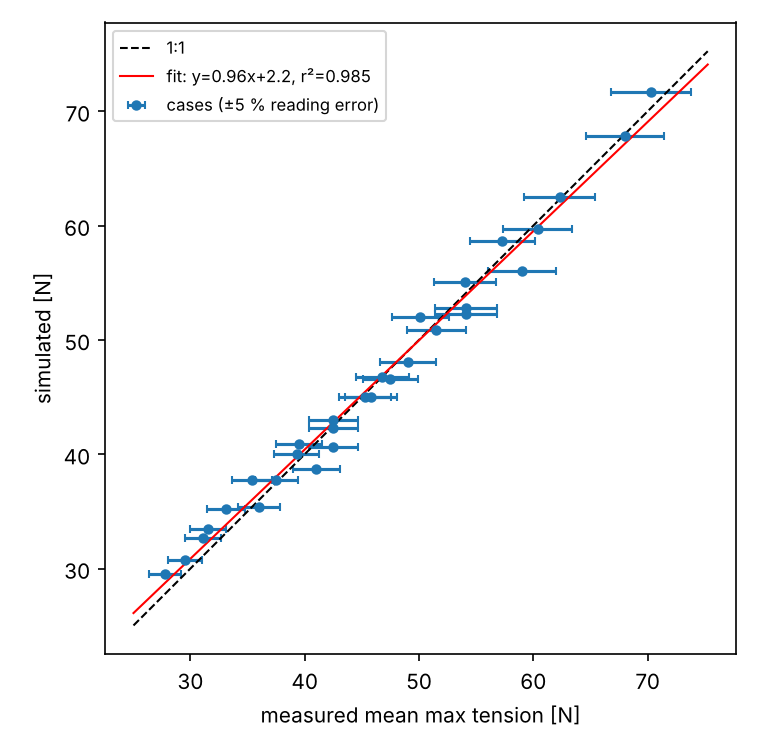
\includegraphics[width=0.62\textwidth]{figures/chalmers_scatter.png}
\caption{Chalmers grid: simulated against measured maximum tension.}\label{fig:chalmers}
\end{figure}

\subsection{Paredes buoy \cite{paredes2016}}
A cylindrical buoy ($m=35.5$\,kg) moored by three legs in three configurations: CON1 (rope with floater), CON2 (with clump weight) and CAT (chain catenary). No coefficient was adjusted; chain hydrodynamic coefficients were applied to the rope (an assumption).
\begin{table}[h]
\centering\small
\begin{tabular}{p{5.2cm}p{4.2cm}p{4.2cm}}
\toprule
Quantity & Model & Measured \\
\midrule
Free heave period & 1.0997\,s & $1.112\pm0.006$\,s ($-1.1\,\%$) \\
Free pitch period & 1.0979\,s & $1.170\pm0.005$\,s ($\mathbf{-6.2\,\%}$) \\
Leg tension CON1 / CON2 / CAT & 2.75 / 10.9--11.0 / 2.93\,N & 2.8--3.1 / 10.6--11.0 / 3.0--3.1\,N \\
Draft change CON1 / CON2 / CAT & +0.6 / +12.9 / +3.4\,mm & +1 / +13 / +4\,mm \\
Surge stiffness vs.\ Fig.~5.21 & CON2 within 3\,\%; CAT 7--10\,\% low; \textbf{CON1 15--19\,\% low} & read by eye, $\pm1.5$\,N/m \\
Damped surge period CON1 / CON2 / CAT & 9.286 / 9.207 / 9.349\,s & 8.561 / 9.22 / 9.14\,s \\
\bottomrule
\end{tabular}
\caption{Paredes buoy: free decay, statics and surge decay (no tuning).}\label{tab:paredes}
\end{table}
The statics agree within the measurement error. The pitch period disagrees ($-6.2\,\%$; the thesis' own total inertia reproduces $1.170$\,s but is derived from that test), and the CON1 stiffness is very sensitive to the rope length: a $1.5\,\%$ length change moves the stiffness by $13\,\%$, so the disagreement lies within the geometric uncertainty of the as-built model.

\paragraph{Regular waves ($T=1.3$ and $1.4$\,s).} With the body coefficients of the thesis (Table~3.4) and Wheeler stretching on the lines, heave is $10$--$21\,\%$ low in 6/6 cases (all within the 25\,\% criterion fixed in advance), pitch meets the 30\,\% criterion in 3/6 (CAT $35$--$50\,\%$ low), and surge is over-predicted by $14\,\%$ up to a factor three. The measured surge RAO has a sharp minimum near $T=1.3$\,s that neither the moored model nor the free hull reproduces. The wave module itself is verified to $10^{-6}$--$10^{-12}$ against closed forms. We regard the wave response as \emph{not validated}.

\subsection{Azcona et al.\ submerged chain \cite{azcona2017}}
A 21\,m chain in a 5\,m deep basin with the fairlead driven horizontally ($T=1.58$, 3.16, 4.74\,s). The amplitude in Table~1 of the paper ($0.25$\,m) was interpreted as peak-to-peak ($\pm0.125$\,m), consistent with the axes of the paper's figures; with $0.25$\,m as the amplitude the snap case would be $268$\,N against $44.5$\,N measured. Static fairlead tension: $8.199$ vs.\ $8.13$\,N ($+0.9\,\%$) and $15.02$ vs.\ $14.48$\,N ($+3.7\,\%$, equivalent to a $2.4$\,cm anchor shift).
\begin{table}[h]
\centering\small
\begin{tabular}{llrrr}
\toprule
Config. & $T$ [s] & Model max [N] & Measured [N] (by eye, $\pm0.5$) & Diff.\ \\
\midrule
1 & 1.58 & 15.12 & 14.5 & $+4.3\,\%$ \\
1 & 3.16 & 10.23 & 9.8 & $+4.4\,\%$ \\
1 & 4.74 & 9.35 & 9.2 & $+1.6\,\%$ \\
2 & 1.58 (snap) & 57.37 & 44.5 & $\mathbf{+28.9\,\%}$ \\
2 & 3.16 & 25.07 & 23.5 & $+6.7\,\%$ \\
2 & 4.74 & 20.35 & 19.5 & $+4.4\,\%$ \\
\bottomrule
\end{tabular}
\caption{Azcona et al.: maximum fairlead tension (60 segments).}\label{tab:azcona}
\end{table}
Five of six cases meet the $\pm8\,\%$ criterion fixed in advance. The snap case is not a converged number: it spans $48$--$67$\,N across discretisations and moves by $-10$ to $-20\,\%$ with physical inputs the paper does not pin down (anchor position, friction, internal damping). We can claim agreement for this case only to within about $+10$--$25\,\%$.

\subsection{Lopez-Olocco et al.\ clump-weight chain \cite{lopezolocco2022}}
A 27\,m studless chain (EA $=3.416\times10^5$\,N) at 6.5\,m depth, anchor distance 25\,m, fairlead on a horizontal circle of radius 0.125--0.225\,m with period 2.8--5.5\,s; a clump (122\,g, 80\,cm$^3$) at $L_s/3$ (CW1) or $L_s/2$ (CW2) from the fairlead. Measured maxima and minima are tabulated in the paper (Tables 8 and 9) and were transcribed from its text layer. Soil and internal-damping parameters are the paper's (Table 7; $\beta=0.0007$\,s, zero friction); nothing was tuned.
\begin{table}[h]
\centering\small
\begin{tabular}{lrrrrr}
\toprule
Config. & Cases & Max, mean diff. & Max, worst & Min, mean $|\Delta|$ [N] & Min, worst [N] \\
\midrule
No clump & 35 & $+2.04\,\%$ & $+4.83\,\%$ & 0.071 & 0.215 \\
CW1 & 9 & $+0.76\,\%$ & $+2.32\,\%$ & 0.453 & 0.911 \\
CW2 & 9 & $-1.81\,\%$ & $-3.70\,\%$ & 0.174 & 0.372 \\
\bottomrule
\end{tabular}
\caption{Lopez-Olocco et al.: maximum and minimum fairlead tension (60 segments without clump, 81 with).}\label{tab:lopez}
\end{table}
The load-cell accuracy is about $\pm0.18$\,N, so the clump-free minima are within instrument accuracy. Static pretension at 25\,m is $11.48$\,N (no clump), $12.17$\,N (CW1) and $12.27$\,N (CW2); the paper reports a CW2 rise of about $10\,\%$ whereas the model gives $+6.9\,\%$, so the static effect of the clump is somewhat under-predicted for a reason not yet isolated. The clump tangential drag coefficient ($1.17$) is assumed (not in the source); for CW1 at $A=0.225$\,m, $T=2.8$\,s (baseline $24.87$\,N, measured $24.31$\,N), $C_{dt}=0.8$ and $1.5$ and no added mass give $24.78$, $24.96$ and $25.00$\,N. Only 53 of the 105 cases were run, the clump cases are not converged in segment count, and one tabulated value (A $=0.150$\,m, CW2, $T=5.0$\,s: $15.72$\,N) appears to contain a typographical error and was not used.

\section{Discussion}
\paragraph{What the evidence supports.} For taut-to-snapping chains driven at the fairlead, the model reproduces maximum fairlead tension to within a few percent for most cases across three independent experiments, with coefficients taken from the sources. Static properties of a three-leg buoy mooring agree within the stated measurement uncertainty.

\paragraph{What it does not support.} (i) Snap loading with total loss of tension is not resolved better than $+10$--$25\,\%$. (ii) Wave-driven motions of the moored buoy are not reproduced (surge in particular), and the potential causes (hydrodynamic coefficient set, reference point, second-order effects) are untested. (iii) The coverage is limited to chains and one polyester rope at laboratory scale; no full-scale, multi-line platform or synthetic-rope data have been compared. The code does not yet include viscoelastic or non-uniform rope properties.

\paragraph{Evidence quality.} Several reference values are digitised or read by eye (Chalmers chart $\pm5\,\%$; Azcona figures $\pm0.5$\,N; Paredes figures), which limits the discrimination of small model errors; the Chalmers rotation sense was inferred after a mismatch; two interpretation choices (Azcona amplitude, Lopez-Olocco clump drag) were required.

\section{Limitations}
Perfectly flexible cable (no bending or torsion, no VIV); small-angle rigid-body dynamics with constant $\mathbf A,\mathbf B$; linear waves only, with line submergence evaluated at the still-water level; flat seabed with a spring--damper; explicit coupling whose body step is limited to about $0.5$--$0.9$ of $2/\omega_s$; a single rigid body; uniform properties along each line.

\section{Conclusions and outlook}
A newly written lumped-mass solver with a coupled 6-DOF body reproduces fairlead tension in three chain experiments to a few percent without tuning, and the paper documents where it fails. Planned work: validation against the NREL/NLR 1:100 mooring data and the OC5 data, which would provide multi-line and larger-scale evidence; a nonlinear/viscoelastic rope law; and a convergence study of snap events with adaptive time stepping. \todo{revise once additional experimental data have been compared}

\section*{Acknowledgements}
Software development, numerical experiments and the drafting of this manuscript were carried out with the assistance of the AI system Claude (Anthropic). The author is responsible for the content; the AI system is not an author. \todo{check the disclosure wording required by the target journal}

\begin{thebibliography}{9}
\bibitem{paredes2016} Paredes, G.M. (2016). \emph{Study of mooring systems for offshore wave energy converters}. PhD thesis. \todo{verify institution and year}
\bibitem{bergdahl2016} Bergdahl, L., Eskilsson, C., Palm, J. (2016). Dynamic mooring analysis validated against a chain test. \emph{J.\ Mar.\ Sci.\ Eng.} 4(1):5. \todo{verify title}
\bibitem{azcona2017} Azcona, J., Munduate, X., Gonz\'alez, L., Nygaard, T.A. (2017). Experimental validation of a dynamic mooring lines code with tension and motion measurements of a submerged chain. \emph{Ocean Eng.} 129:415--427.
\bibitem{lopezolocco2022} Lopez-Olocco, T. et al.\ (2022). \emph{J.\ Mar.\ Sci.\ Eng.} 10(5):676. \todo{full author list and title}
\bibitem{hall2015} Hall, M., Goupee, A. (2015). Validation of a lumped-mass mooring line model with DeepCwind semisubmersible model test data. \emph{Ocean Eng.} 104:590--603.
\end{thebibliography}
\end{document}
